%%
%% This is file `tikzposter-example.tex',
%% generated with the docstrip utility.
%%
%% The original source files were:
%%
%% tikzposter.dtx  (with options: `tikzposter-example.tex')
%% 
%% This is a generated file.
%% 
%% Copyright (C) 2014 by Pascal Richter, Elena Botoeva, Richard Barnard, and Dirk Surmann
%% 
%% This file may be distributed and/or modified under the
%% conditions of the LaTeX Project Public License, either
%% version 2.0 of this license or (at your option) any later
%% version. The latest version of this license is in:
%% 
%% http://www.latex-project.org/lppl.txt
%% 
%% and version 2.0 or later is part of all distributions of
%% LaTeX version 2013/12/01 or later.
%% 








 \documentclass[17pt, a1paper, portrait, margin=0mm, innermargin=1mm,
     blockverticalspace=3mm, colspace=5mm, subcolspace=5mm]{tikzposter} %Default values for poster format options.

\tikzposterlatexaffectionproofoff %shows small comment on how the poster was made at bottom of poster
\usepackage{exscale}
\usepackage{listings}
\usepackage[hidelinks]{hyperref}
\usepackage{wrapfig}
\usepackage[backend=biber]{biblatex}
\addbibresource[datatype=bibtex]{dmposter.bib}


 % Commands
 \newcommand{\bs}{\textbackslash}   % backslash
 \newcommand{\cmd}[1]{{\bf \color{red}#1}}   % highlights command
 \usepackage{float}
 \floatstyle{boxed}
 \restylefloat{figure}

 % Title, Author, Institute
\title{Can Twitter User's Moods Predict the Stock Market?}
\author{Aaron Gonzales and Adam Delora}
\institute{Department of Computer Science, University of New Mexico} 
%\titlegraphic{blah}

 % -- PREDEFINED THEMES ---------------------- %
 % Choose LAYOUT:  Default, Basic, Rays, Simple, Envelope, Wave, Board, Autumn, Desert,
\usetheme{Simple}
%\usecolorstyle[colorPalette=BrownBlueOrange]{Germany}


 \begin{document}

 \maketitle[width=55cm, titletotopverticalspace=0.0cm]

 \begin{columns}%blocks will be placed into columns
   \column{.50}
%%%%%%%%%%%%%%%%new block%%%%%%%%%%%%%%%%%%%%%%%%%%%%%%%%%%%%
   \block{Background}{
     \begin{itemize}
       \item Twitter is a microblogging service with 284 million monthly
         active users who post 500 million updates (``tweets'') per day.
       \item Latent Semantic Indexing is a technique used to summarize
         words (documents) into representative ideas similar to principle
         component analysis.
       \item The AFINN semantic indexing database (\cite{ANEW}) assigns coded valence
         values to common words to allow quantification of a set of word's
         ``mood''.
     \end{itemize}
   }
%%%%%%%%%%%%%%%%new block%%%%%%%%%%%%%%%%%%%%%%%%%%%%%%%%%%%%
   \block{Methods}{
     We collected tweets using the public Twitter Streaming RESTful API
     over 2014-10-17 \textemdash 2014-11-09 by tracking words that related
     to various tech stocks indexed by NASDAQ.           
     \begin{tikzfigure}[Several examples of de-identified tweets from our
       dataset] 
       \label{fig:tweets}
       \begin{itemize}
         \item \small{Maine nurse defies Ebola quarantine order by taking bike ride.
           http://t.co/eERINkm3AQ via @indystarJ}
         \item \small{Tim Cook: Apple CEO Says 'Being Gay Is One Of God's
             Greatest Gifts' Earlier today, the chief executive of
             Apple,\ldots \url{http://t.co/zIXb2HbDmd}}
         \item \small{ Meet the Swedish twin sisters who want to be
             'identical artificial dolls' \url{http://t.co/77eA3esaQa}}
         \item \small{Last Christmas I got a black iPhone it was the
           worst Christmas present ever, I wanted a white one. I mean I'm
           not\ldots \url{http://t.co/jhP9ODs3QK}}
       \end{itemize}
         \tiny{\textcolor{white}{blah}}
     \end{tikzfigure}
          
    %\begin{wrapfigure}[6]{l}{0.33\linewidth}
     \begin{tikzfigure}[Kewords tracked] \label{fig:keywords}
       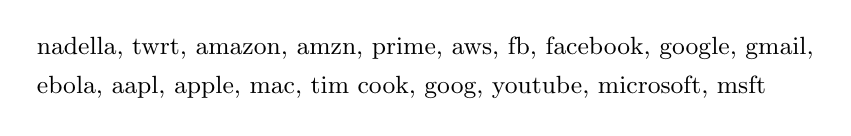
\begin{tikzpicture}
         \node[anchor=north west] (note2) at (0,0)
         { \small{ebola, aapl, apple, mac, tim cook, goog,
           youtube, microsoft, msft }};
         \node[anchor=north west] (note2) at (0,0.5)
         { \small{nadella, twrt, amazon, amzn, prime, aws, fb,
         facebook, google, gmail,}};
       \end{tikzpicture}
     \end{tikzfigure}
    %\end{wrapfigure}
     NASDAQ market data was collected over a slightly longer period, 2014-08-30
     - 2014-11-09. Tweets were preprocessed to remove common stopwords. Latent semantic indexing
     was performed using Gensim \cite{rehurek_lrec}  on one-hour bag-of-words bins of
     tweets, giving a total of xxx hours included in analysis. Each hour's
     LSI topics were scored using the AFINN database, resulting in a single
     number indicating semantic valence for each hour. The LSI score was
     smoothed using rolling means and assessed
     for periodicity.  Semantic data was combined with the stock data and
     standardized for
     visualization and analysis. A model was created using vector autoregression (VAR) to assess 	the predictive power of the semantic data against the
     stock data.

     Within an hour LSI would provide a set of topics like the following topic from 14:00-15:00
     on 2014-10-16:
     \begin{tikzfigure}[Two LSI topics]
       \label{tab:topics}
       \begin{tabular}{|c|c|c|c|c|c|c|c|c|c|}
         \hline
         scientists & are   & about & do    & don't & over  & say   & climate & it    & panic \\ 
         \hline
         0.416      & 0.219 & 0.217 & 0.216 & 0.214 & 0.211 & 0.209 & 0.209   & 0.209 & 0.208 \\ 
         \hline
         %\end{tabular}
         %\begin{tabular}{|c|c|c|c|c|c|c|c|c|c|}
         \hline
         on    & is     & get    & from  & ebola  & i      & google & it     & really & liked \\ 
         \hline
         0.586 & -0.315 & -0.217 & 0.165 & -0.140 & -0.129 & -0.126 & -0.122 & -0.117 & 0.208 \\ 
         \hline
       \end{tabular}
     \end{tikzfigure}
   } 
%%%%%%%%%%%%%%%%new block%%%%%%%%%%%%%%%%%%%%%%%%%%%%%%%%%%%%
         \block{Summary Statistics}{
           %\begin{wrapfigure}{l}{0.40\linewidth}
             %\begin{tikzfigure}[Rolling Means of LSI score] \label{fig:summary}
             %%\includegraphics[width=4in]{figures/lsi_rolling_means.png}
               %\includegraphics[width=0.99\linewidth]{figures/lsi_rolling_means.png}
             %\end{tikzfigure}
           %\end{wrapfigure}
           \begin{itemize}
             \item \small{Total tweets collected: 84 million}
             \item \small{Total hours analyzed: 218}
             \item \small{Number of tweets per hour: 205,200; std 71,700}
             \item \small{Mean semantic score:  4.78; std 1.39}
           \end{itemize}
           blah
           %\begin{wrapfigure}{l}{0.8\linewidth}
           \begin{tikzfigure}[Word clouds generated from topics on 2014-10-30,
             11:00-12:00 and 12:00 - 13:00]
             \label{fig:wordcloud}
             {\includegraphics[width=0.35\linewidth]{../analysis/img170.png}}
             {\includegraphics[width=0.35\linewidth]{../analysis/img173.png}}
             %{\includegraphics[width=0.46\linewidth]{figures/lsi_rolling_means.png}}
           \end{tikzfigure}
         %\end{wrapfigure}
         }

%%%%%%%%%%%%%%%%%%%%%%%%%%%%%%%%%%%%%%%%%%%%%%%%%%%%%%%%%%
%%%%%%%%%       new col         %%%%%%%%%%%%%%%%%%%%%%%%%%
%%%%%%%%%%%%%%%%%%%%%%%%%%%%%%%%%%%%%%%%%%%%%%%%%%%%%%%%%%

         \column{.5}
%%%%%%%%%%%%%%%%new block%%%%%%%%%%%%%%%%%%%%%%%%%%%%%%%%%%%%
         \block{Stocks}{
           \begin{tikzfigure}[Rolling means of z-scored LSI score and stock prices per hour]
             \label{fig:means}
             \includegraphics[width=8in]{figures/stock_plot_with_lsi}
           \end{tikzfigure}
         }
%%%%%%%%%%%%%%%%new block%%%%%%%%%%%%%%%%%%%%%%%%%%%%%%%%%%%%
   \block{Results}{
   %\begin{wrapfigure}{l}{0.8\linewidth}
    \begin{tikzfigure}[Impulse Response analysis of LSI score change]
     \label{fig:impulseresponse}
     \includegraphics[width=7in]{figures/impulse_responses}
   \end{tikzfigure}
   %\end{wrapfigure}
    VAR models are used to model multivariate time
    series. They describe a set of $k$ variables as a linear function of
    their previous values. A $p$-th order VAR model is denoted by
    $y_t = c + A_1 y_{t-1} + A_2 y_{t-2} + \cdots + A_p y_{t-p} + e_t$.
    VAR models are often used with a lag parameter that operates on the
    elements of a time series to produce the previous element. We determined
    the lag order by employing an information criteria-based order selection
    which led us to use a lag of 1 hour in the model. Python/Statsmodels
    \cite{statsmodels2010} were used for analysis.

   Our VAR model indicated LSI score was a significant predictor of Amazon
   $(t = -2.312, p = 0.023)$, Facebook $(t = -2.527, p = 0.013)$, and Twitter
   $(t = 2.566, p = 0.012)$ and Granger's causality test concluded that there
   was a causal effect of LSI score on Amazon $(f = 9.68, p = 0.02)$ and
   Google $(f = 8.584039, p = 0.003)$.
   }

   \block{References and Acknowledgements}{
     \renewcommand*{\bibfont}{\footnotesize}
     \printbibliography
   }

 \end{columns}


\end{document}




\endinput
%%
%% End of file `tikzposter-example.tex'.
